\section{Ausweichen}
\begin{center}
    \begin{tikzpicture}[node distance = 3cm, auto]
            % Nodes
        \node [block] (init) {\hypertarget{ausweichen}{Wird angegriffen}} ;
        \node [decision, below of=init] (erschw) {Gezielt Ausw.? (Ausw. I nötig)};
        \node [decision, below left = 3cm of erschw] (gezielt) {Erschw. aus DK x2};
        \node [block, below left of=gezielt] (bestanden) {Entgeht Angriff};
        \node [block, below right of=gezielt] (verkackt) {Wird getroffen, INI -2};
        \node [decision, below right = 3cm of erschw] (ungezielt) {Erschw.};
        \node [block, below left of=ungezielt] (bestanden2) {Entgeht Angriff, INI -4, \textit{Position}};
        \node [block, below right of=ungezielt] (verkackt2) {Wird getroffen, INI -4, \textit{Position}};

            % Edges
        \path [line] (init) -> (erschw);
        \path [line] (erschw) -> (gezielt);
        \path [line] (gezielt) -> (bestanden);
        \path [line] (gezielt) -> (verkackt);
        \path [line] (erschw) -> (ungezielt);
        \path [line] (ungezielt) -> (bestanden2);
        \path [line] (ungezielt) -> (verkackt2);
    \end{tikzpicture}\\
\end{center}
\begin{center}
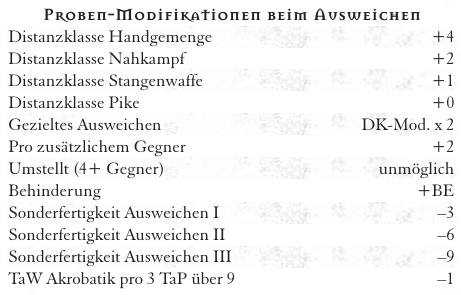
\includegraphics[width=\linewidth]{Kampf/Ausweichen/img/erschwernis.png}
\end{center}